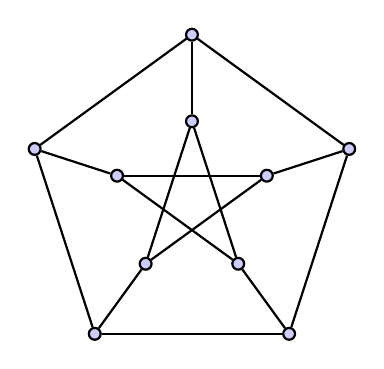
\begin{tikzpicture}
    \tikzset{
        vert/.style = {
            draw,
            thick,
            circle,
            inner sep = 0pt,
            minimum size = 0.15cm,
            fill = blue!20
        }
    }
    
    \def\R{2.1}
    \def\r{1}
    \foreach \a in {0, 1, ..., 4}{
        \node[vert] (a\a) at (90 - \a * 360 / 5:\R) {};
        \node[vert] (b\a) at (90 - \a * 360 / 5:\r) {};

        \draw[thick] (a\a) -- (b\a);

    }

    \foreach \a [
        evaluate = \a as \i using {int(Mod(5 + \a - 1, 5))},
        evaluate = \a as \j using {int(Mod(\a + 2, 5))}] in {0, ..., 4}{
            \draw[thick] (a\a) -- (a\i);
            \draw[thick] (b\a) -- (b\j);
    }
    

\end{tikzpicture}